\documentclass{book}
\usepackage{blindtext}
\usepackage[T1]{fontenc}
\usepackage[utf8]{inputenc}
\usepackage{booktabs}
\usepackage{csvsimple}
\usepackage{graphicx}
\usepackage{wrapfig}
\usepackage[a4paper,width=150mm,top=25mm,bottom=25mm,bindingoffset=10mm,headsep=10mm]{geometry}
\usepackage{fancyhdr}
\renewcommand{\headrulewidth}{1pt}
\pagestyle{fancy}
\fancyhead[RO,LE]{Chapter \thechapter}
\graphicspath{./outros}

\title{Apresentacao para o preparo da Historia}
\author{Lucas Tatsuya Tanaka}
\date{\today}


\begin{document}
\maketitle
\tableofcontents

\vspace*{\fill} 
\begin{quote} 
\centering 
\Large {Tudo aqui presente pode ser alterado ou atualizado, tendo em vista a diversao de todos
\huge {caso tenha duvidas me contata ai }}

\end{quote}
\vspace*{\fill}



\part{Apresentacao inicial}
\chapter{Quais sao os elementos que guiam essa historia?}
\begin{itemize}
    \item A revitalizacao do magico no mundo
    \item A vivencia na era da mudanca 
    \item O mundo atual esta preste a ter grandes mudancas a qualquer momento
\end{itemize}


\chapter{O que eh preciso saber sobre o mundo?}
\begin{itemize}
    \item O mundo e dividido por castas 
    \item Os antigos deuses primordiais sao dragoes
    \item O mundo e velho 
    \item O mundo esta vivendo uma era de retorno do mistico 

\end{itemize}
\section{Deuses ancestrais}
\begin{itemize}
    \item Azcoda o deus do conhecimento
    \item Venada o deus da natureza
    \item Amtem o deus da tempestade
    \item Verguemo o deus do conflito
    \item Roenmo o deus da comunicacao
\end{itemize}
\section*{Academias de Magia}    
As academias de magia surgem da valorizacao de seres que tinhamm alguma habilidade magica 
e como uma centralizacao de conhecimento visto que a presenca de usuarios de magias se 
tornou um comodite muito importante para as nacoes
\section*{Companhia de coletas}
Companhis de coletas sao locais ao qual as pessoas vao quando necessitam de algo em que 
necesite de um trabalho mais especializado ou algum tipo de servico mais especializado
e nao sabem muita das vezes a quem consultar (uma dita guilda no mundo de Kuara)

\part{Uma breve introducao as Racas}

\chapter{Anao}
 
% \begin{wrapfigure}{r}{0.5\textwidth}
%     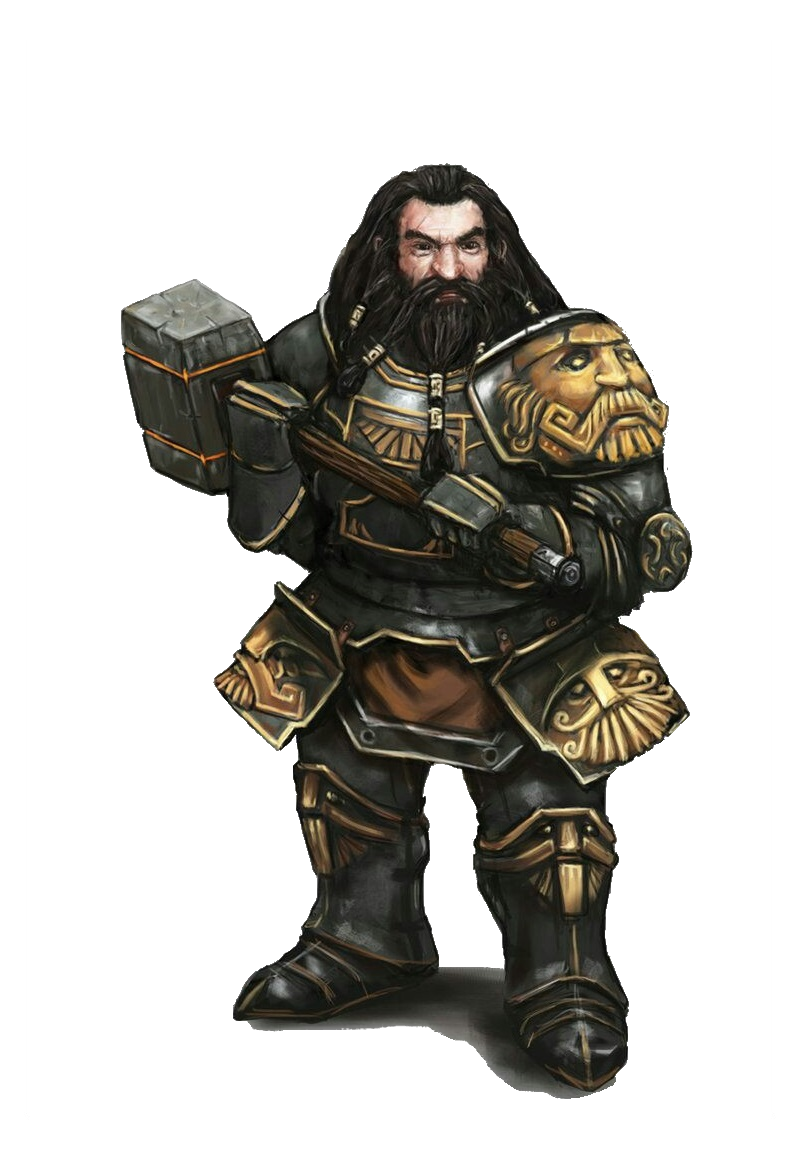
\includegraphics[width=1\linewidth]{outros/dwarf.png}
%     \caption{caption1}\label{fig:wrapfig}
% \end{wrapfigure}

Seres de estatura media a baixa com um tipo de construcao corporal densa e forte 

\section{Tracos Raciais}
\begin{itemize}
    \item \textbf{Aumento no valor de habilidade:} +2 em constituicao, +2 em forca
    \item \textbf{Idade:} Anões tornam-se maduros na mesma proporção que os humanos, mas são
          considerados jovens até atingirem a idade de 50 anos. Em média, eles vivem 350 anos.
    \item \textbf{Tamanho:} Anões estão entre 1,20 e 1,50 metro de altura e pesam cerca de 
          75 kg. Seu tamanho é Médio
    \item \textbf{Deslocamento:} Seu deslocamento base de caminhada é de 7,5 metros. Seu 
          deslocamento
          não é reduzido quando estiver usando armadura pesada.
       \item \textbf{Resiliência Anã:} Você possui vantagem em testes de resistência contra    
          venenos  e resistência contra dano de veneno (explicado no capitulo 9)
    \item \textbf{Treinamento Anão em Combate:} Você tem proficiência com machados de 
          batalha, machadinhas, martelos leves e martelos de guerra 
    \item \textbf{Proficiência com Ferramentas} Você tem proficiência em uma ferramenta de 
          artesão à sua escolha entre: ferramentas de ferreiro, suprimentos de cervejeiro ou 
          ferramenta de pedreiro 
    \item \textbf{Especialização em Rochas} Sempre que você realizar um teste de Inteligência
          (História) relacionado à origem de um trabalho em pedra, você é considerado
          proficiente na perícia História e adiciona o dobro do seu bônus de proficiência 
          ao teste, ao invés do seu bônus de proficiência normal.
    \item \textbf{Idiomas} Você pode falar, ler e escrever Comum e alto.
    \item \textbf{Treinamento Anão com Armaduras} Você adquire proficiencia em armaduras leves 
          e medias
\end{itemize}

\section{Passado}
O passado Anao esta cercada por antigos imperios, des de sua existencia a sua total decadencia
glorias passadas e uma historia de lutas e guerras 
\section{Modernidade}
A atualidade dos anoes modernos vivem uma cultura dissolvida e integrada a outras sociedades 
atingindo as mais diversas das classes sociais des do escravo ate o maior politicos, porem 
nunca atingindo o estado de nobreza como as 3 outras racas (Tiefilings, Draconatos e Elfos) 

\chapter{Elfo da floresta}
Seres antigos de estatura media de orelhas pontudas e corpo esguio
% imagem de um elfo comum
\section{Tracos Raciais}
\begin{itemize}
    \item \textbf{Aumento no valor de Habilidades}: +2 em destreza, +1 em sabedoria 
    \item \textbf{Idade}: Embora os elfos atinjam a maturidade física com praticamente a mesma 
          idade dos humanos, a compreensão élfica da idade adulta vai além da maturidade 
          física, abrangendo sua experiência sobre o mundo. Um elfo tipicamente assume 
          a idade adulta e um nome adulto com cerca de 100 anos de idade e pode viver
          750 anos.
    \item \textbf{Tamanho:} Elfos medem entre 1,50 a 1,80 metro de altura e possuem 
          constituição delgada. Seu tamanho é Médio.
    \item \textbf{Deslocamnto} Seu deslocamento base de caminhada e 9 metros
       \item \textbf{Sentidos Aguçados:} Você tem proficiência na perícia Percepção.
    \item \textbf{Ancestral de Venada:} Você tem vantagem nos testes de resistência para 
          resistir  a ser enfeitiçado e magias não podem colocá-lo para dormir.
    \item \textbf{Transe} Elfos não precisam dormir. Ao invés disso, eles meditam 
          profundamente, permanecendo semiconscientes, durante 4 horas por 
          dia. (A palavra em idioma comum para tal meditação é `transe`.) Enquanto
          medita, um elfo é capaz de sonhar de certo modo. Esses sonhos na verdade 
          são exercícios mentais que se tornam reflexos através de anos de prática.
          Depois de descansar dessa forma, você ganha os mesmos benefícios que um
          humano depois de 8 horas de sono.
    \item \textbf{Treinamento Élfico com Armas:} Você possui proficiência com espadas 
          longas, espadas curtas, arcos longos e arcos curtos.
    \item \textbf{Pés Ligeiros:} Seu deslocamento base de caminhada aumenta para 10,5 metros.

    \item \textbf{Máscara da Natureza} Você pode tentar se esconder mesmo quando você está
          apenas levemente obscurecido por folhagem, chuva forte, neve caindo, névoa ou 
          outro fenomeno natural.
    \item \textbf{Idiomas:} voce pode ler e escrever elfico e comum 
\end{itemize} 
\section{Passado}
O passado dos elfos da floresta esta diretamente ligado aos Altos elfos da floresta de 
Cac~apava, estes descendem dos primeiros elfos a sairem da mesma floresta para uma exploracao
das regioes fora da floresta criando novos reinados e imperios em outras regioes.
\section{Modernidade}
A autualidade do elfo no mundo de Kuara (aonde tange a atual campanha) esta ligada as nobrezas 
e os autos estratos das classes sociais, atualmente ocupam o status de um `raca nobre' nos 
atuais reinos draconicos 

\chapter{Elfo da montanha}
    Seres antigos de estatura media de orelhas pontudas e corpo esguio
\section{Tracos Raciais}
\begin{itemize}
    \item \textbf{Aumento no valor de Habilidades}: +2 em destreza, +1 em Forca
    \item \textbf{Idade}: Embora os elfos atinjam a maturidade física com praticamente a mesma 
          idade dos humanos, a compreensão élfica da idade adulta vai além da maturidade 
          física, abrangendo sua experiência sobre o mundo. Um elfo tipicamente assume 
          a idade adulta e um nome adulto com cerca de 100 anos de idade e pode viver
          750 anos.
    \item \textbf{Tamanho:} Elfos medem entre 1,50 a 1,80 metro de altura e possuem 
          constituição delgada. Seu tamanho é Médio.
    \item \textbf{Deslocamnto} Seu deslocamento base de caminhada e 9 metros
       \item \textbf{Sentidos Aguçados:} Você tem proficiência na perícia Percepção.
    \item \textbf{Ancestral de Venada:} Você tem vantagem nos testes de resistência para 
          resistir  a ser enfeitiçado e magias não podem colocá-lo para dormir.
    \item \textbf{Transe} Elfos não precisam dormir. Ao invés disso, eles meditam 
          profundamente, permanecendo semiconscientes, durante 4 horas por 
          dia. (A palavra em idioma comum para tal meditação é `transe`.) Enquanto
          medita, um elfo é capaz de sonhar de certo modo. Esses sonhos na verdade 
          são exercícios mentais que se tornam reflexos através de anos de prática.
          Depois de descansar dessa forma, você ganha os mesmos benefícios que um
          humano depois de 8 horas de sono.
    \item \textbf{Treinamento de armas da montanha:} Você possui proficiência com espadas 
          curtas, longas, machadinhas, machados, lanca e gladio
    \item \textbf{Corredor de Obstrucoes:} Enquanto movendo em seu turno voce consegue ignorar 
          ate 3 metros de terreno difil

    \item \textbf{Escalador Natural:}voce tem proficiencia em atletismo e acrobacia
    \item \textbf{Idiomas:} voce pode ler e escrever alto e comum 
\end{itemize}
\section{Passado}
O passado dos elfos da montanha estao ligados aos altos elfos da floresta de Cacapava e dos 
primeiros exploradores elfos do oeste que descidiram fazer a passagem para o outro 
continente pelos complexos de montanhas de Araxa gerando em seu caminhos
civilizacoes e imperios 
\section{Modernidade}
A atualidade dos Elfos de Montanha em Kuara (aonde tange a atual campanha) eh incomum
nos reinos draconicos nao eh muito comum ver um elfo de montanha, porem aqueles que se vem 
geralmente esta ligada a outros paises e poucas vezes ligados com a nobreza dos reinos 
draconicos e suas altas classes 

% Os elfos da montanha sao Nobres nos reinos draconicos ?
% Eles vivem uma sociedade diferente dos elfos da floresta nos reinos Draconicos?
% tem se poucos ? muitos? 
% sao ligados a qual nacao ?
% Esta raca tem relevancia pra historia ? 
% Eles realmente falam elfico?

\chapter{Elfo do deserto}
    Seres antigos de estatura media de orelhas pontudas e corpo esguio
% colocar uma imagem do elfo do deserto
\section{Tracos Raciais}
\begin{itemize}
    \item \textbf{Aumento no valor de Habilidades}: +2 em destreza, +1 em constituicao
    \item \textbf{Idade}: Embora os elfos atinjam a maturidade física com praticamente a mesma 
          idade dos humanos, a compreensão élfica da idade adulta vai além da maturidade 
          física, abrangendo sua experiência sobre o mundo. Um elfo tipicamente assume 
          a idade adulta e um nome adulto com cerca de 100 anos de idade e pode viver
          750 anos.
    \item \textbf{Tamanho:} Elfos medem entre 1,50 a 1,80 metro de altura e possuem 
          constituição delgada. Seu tamanho é Médio.
    \item \textbf{Deslocamnto} Seu deslocamento base de caminhada e 9 metros
       \item \textbf{Sentidos Aguçados:} Você tem proficiência na perícia Percepção.
    \item \textbf{Ancestral de Venada:} Você tem vantagem nos testes de resistência para 
          resistir  a ser enfeitiçado e magias não podem colocá-lo para dormir.
    \item \textbf{Transe} Elfos não precisam dormir. Ao invés disso, eles meditam 
          profundamente, permanecendo semiconscientes, durante 4 horas por 
          dia. (A palavra em idioma comum para tal meditação é `transe`.) Enquanto
          medita, um elfo é capaz de sonhar de certo modo. Esses sonhos na verdade 
          são exercícios mentais que se tornam reflexos através de anos de prática.
          Depois de descansar dessa forma, você ganha os mesmos benefícios que um
          humano depois de 8 horas de sono.
    \item \textbf{Guardiao Nomade:}voce tem proficiencia com lanca, simitarra, arco curto e  
        pique
    \item \textbf{Sobrevivente Engenhoso:}Voce tem proficiencia na habilidade sobrevivencia
    \item \textbf{Nascido do Deserto:}voce e naturalmente adaptado a climas quentes 
    \item \textbf{Miragen:}Voce consegue castar a habilidade blur usando esta habilidade, ela 
          eh regenerada apos um longo descanco 
     \item \textbf{Idiomas:} voce pode ler e escrever ancestral e comum 

\end{itemize}
\section{Passado}
A antiguidade desta raca esta ligada aos altos elfos de Cacapava e aos primeiros exploradores 
do oeste que decidiram passar pelo torturoso deserto de ybytata que em sua passagem 
geraram reinos e imperios, durante sua passagem acabaram por entrar em contato com outras 
racas costumes e afins.
\section{Modernidade}
A atualidadae dos elfos do deserto no mundo de Kuara (aonde tange a atual campanha) estao 
ligados a outras nacaoes, e se encontram em pouquissima quantidade nos imperios draconianos 
ocupando locais que tangem a alta classe dos imperios draconicos em sua maioria 

% sao ligados a quais nacoes ?
% tem sua lealdade ligados aos seus lugares de origem ?
% vale a pena colocar ele nahistoria ?
% quais sao seus tracoes culturais?
% eles realmente falam elfico?

\chapter{Hafling pes leves}
    Sao pequenos e ageis seres que sao facilmente mesclados com as pessoas em seu arredor.
    % foto de um halfling
\section{Tracos Raciais}
\begin{itemize}
    \item \textbf{Aumento no valor de Habilidades}: +2 em destreza, +1 em carisma
    \item \textbf{Idade:} Um halfling atinge a idade adulta aos 20 anos e pode chegar a 150    
          anos
    \item \textbf{Tamanho:} Halflings medem cerca de 0,90 metro de altura e pesam 
          aproximadamente 20 kg. Seu tamanho é Pequeno.
    \item \textbf{Deslocamento:} Seu deslocamento base de caminhada é 7,5 metros.
    \item \textbf{Sortudo:} Quando você obtiver um 1 natural em uma jogada de ataque, teste 
          de habilidade ou teste de resistência, você pode jogar de novo o dado e deve 
          utilizar o novo resultado.
    \item \textbf{Bravura:} Você tem vantagem em testes de resistência contra ficar amedrontado
    \item \textbf{Agilidade Halfling} Você pode mover-se através do espaço de qualquer 
          criatura que for de um tamanho maior que o seu.
    \item \textbf{Furtividade Natural:}Voce pode se esconder mesmo quando possuir apenas a 
          cobertura de uma criatura que for no mínimo um tamanho maior que o seu.
    \item \textbf{Idioma:} Voce pode ler e escrever comum e Halfling
\end{itemize} 
\section{Passado}
A antiguidade dos halflings pes leves e desconhecida devido a sua baixa tradicao literaria 
porem os boatos dizem que eles sao uma variacao de humano com elfos e anoes que depois de
anos se tornaram o que hoje eh o halfling
\section{Modernidade}
A atualidade dos Halfling pes leves no mundo atual de Kuara (aonde tange a atual campanha) 
esta ligada a comunidades pequenas e interioranas
em sua grande parte sao seres relaxadas que buscam poucos conflitos porem aqueles que 
fogem tal ideia geralmente sao curiosos e estao ligados aos mais diversos dos trabalhos

\chapter{Hafling robusto}
    Sao pequenos e ageis seres que sao facilmente mesclados com as pessoas em seu arredor.
    % foto de um halfling
\section{Tracos Raciais}
\begin{itemize}
    \item \textbf{Aumento no valor de Habilidades}: +2 em destreza, +1 em constituicao
    \item \textbf{Idade:} Um halfling atinge a idade adulta aos 20 anos e pode chegar a 150    
          anos
    \item \textbf{Tamanho:} Halflings medem cerca de 0,90 metro de altura e pesam 
          aproximadamente 20 kg. Seu tamanho é Pequeno.
    \item \textbf{Deslocamento:} Seu deslocamento base de caminhada é 7,5 metros.
    \item \textbf{Sortudo:} Quando você obtiver um 1 natural em uma jogada de ataque, teste 
          de habilidade ou teste de resistência, você pode jogar de novo o dado e deve 
          utilizar o novo resultado.
    \item \textbf{Bravura:} Você tem vantagem em testes de resistência contra ficar amedrontado
    \item \textbf{Agilidade Halfling} Você pode mover-se através do espaço de qualquer 
          criatura que for de um tamanho maior que o seu.
    \item \textbf{Resiliencia dos Robustos: }Voce tem vantagens em testes de resistencia 
          contra veneno e tem resistencia contra dano de veneno
    \item \textbf{Idioma:} Voce pode ler e escrever comum e Halfling

\end{itemize}
\section{Passado}
A antiguidade dos halflings robustos e desconhecida devido a sua baixa tradicao literaria 
porem os boatos dizem que eles sao uma variacao de humano com elfos e anoes que depois de
anos se tornaram o que hoje eh o halfling
\section{Modernidade}
A atualidade dos Halfling pes leves no mundo atual de Kuara (aonde tange a atual campanha) 
esta ligada a comunidades pequenas e interioranas
em sua grande parte sao seres relaxadas que buscam poucos conflitos porem aqueles que 
fogem tal ideia geralmente sao curiosos e estao ligados aos mais diversos dos trabalhos

\chapter{Humano}
    Apresentam nenhuma individualidade forcas ou fraquezas sao seres com grandes vontades e 
    desejos
\section{Tracos Raciais}
\begin{itemize}
    \item \textbf{Aumento no Valor de Habilidade:} Todos os seus valores de habilidade 
          aumentam em 1.
    \item \textbf{Idade:} Os humanos chegam à idade adulta no final da adolescência e vivem 
          menos de um século.
    \item \textbf{Tamanho:} Os humanos variam muito em altura e peso, podem ter quase 1,50   
          metro ou mais de 1,80 metro.
    \item \textbf{Deslocamento:} Seu deslocamento base de caminhada é 9 metros.
    \item \textbf{Idiomas:} Você pode falar, ler e escrever Comum e outro idioma adicional, à  
          sua escolha. Os humanos normalmente aprendem os idiomas dos povos que
          convivem, incluindo dialetos obscuros. Eles gostam de rechear seu discurso com
          palavras emprestadas de outras línguas: xingamentos orcs, expressões musicais 
          élficas, frases militares anãs e outros.
\end{itemize}
\section{Passado}
A antiguidade dos humanos esta ligada as mais diversas das sociedades des de grandes imperios 
ate pequenas sociedades de nomades sendo presente em grande parte da historia do mundo de Kuara
\section{Modernidade}
A atualidade do Humano no mundo de Kuara (aonde tange a atual campanha) esta ligada a sua 
presenca em diversos dos estratos socias porem com uma porcao de pequena a media devido a 
uma baixa quantida de humanos no mundo de Kuara 

\chapter{Draconato}
Apresentam uma historia riquisima e antiga, estes apresentam aparencias semelhantes a dragoes 
apresentando as mais diversas das cores tamanhos e formas. 
\section{Tracos Raciais}
\begin{itemize}
     \item \textbf{Aumento no Valor de Habilidade:} Força +2, Carisma +1.
     \item \textbf{Idade:} Draconatos jovens crescem rapidamente. Eles caminham horas após 
      nascerem, adquirindo o tamanho e desenvolvimento semelhante a de uma criança humana
      de 10 anos com 3 anos de idade e alcançam a maturidade aos 15. Eles costumam a viver ate 
      os 210 anos de idade 
     \item \textbf{Tamanho:} Os draconatos são mais altos e mais pesados que os humanos, 
         geralmente possuindo mais de 1,80 metro e normalmente pesando mais de 125 kg. Seu 
         tamanho é Médio.
     \item \textbf{Deslocamento:} Seu deslocamento base de caminhada é 9 metros.
     \item \textbf{Ancestral Dracônico:} Você possui um ancestral dracônico. Escolha um tipo 
         de 
       dragão da tabela Ancestral Dracônico. Sua arma de sopro e resistência a dano são
       determinadas pelo tipo de dragão, como mostrado na tabela.
       (A tabela utilizada eh a mesma de Dnd 5ed)

  \item \textbf{Arma de Sopro:} Você pode usar uma ação para exalar energia destrutiva. Seu 
       ancestral dracônico determina o tamanho, formado e tipo de dano que você
       expele. Quando você usa sua arma de sopro, cada criatura na área exalada deve realizar 
       um teste de resistência, o tipo do teste é determinado pelo seu ancestral 
       dracônico. A CD do teste de resistência é 8 + seu modificador de Constituição + seu   
       bônus de  proficiência. Uma criatura sofre 2d6 de dano num fracasso e metade desse dano 
       num sucesso. O dano aumenta para 3d6 no 6° nível, 4d6 no 11° nível e 5d6 no 16° nível.
       Depois de usar sua arma de sopro, você não poderá utilizá-la novamente até completar um
       descanso curto ou longo.
  \item \textbf{Resistencia a Dano:}Voce possui resistencia ao tipo de dano associado ao seu 
      ancestral draconico.
  \item \textbf{Idiomas:}Voce pode falar ler e escrever Comum e Draconico.
\end{itemize}
\section{Passado}
A antiguidade dos draconatos esta ligada a mais antigas sociedades do mundo de Kuara sendo 
uma das primeiras sociedades a comecar a existir no mundo tendo uma disposicao grande pelo 
mundo mas porem concentradas devido a sua organizacao social e religiosa
\section{Modernidade}
A modernidade dos draconatos no mundo de Kuara (aonde tange a atual campanha) esta ligada 
as cidades mais populadas e grandes centros urbanos, devido a sua historia e atual disposicao
social, que se faz presente nas diversas classes sociais altas ocupando um status de `raca 
nobre'

\chapter{Gnomo Floresta}
Seres inventivos e criativos devido a isto estao presentes nos mais diversos dos estratos 
sociais envolvidos em sua maioria com os estudos e descoberta
\section{Tracos Raciais}
\begin{itemize}
    \item \textbf{Aumento no Valor de Habilidade:} +2 em Inteligência, +1 em Destreza.
    \item \textbf{Idade:} Gnomos amadurecem a mesma proporção que os humanos e, a 
          maioria, atinge a idade adulta por volta dos 40 anos. Eles podem viver 
          entre 350 e 500 anos.
    \item \textbf{Tamanho:} Os gnomos tem entre 0,90 e 1,20 metro e seu peso medio e de
          20kg  seu tamnho e pequeno
    \item \textbf{Deslocamento:} Seu deslocamento base de caminhada é 7,5 metros.
     \item \textbf{Esperteza Gnômica:} Você possui vantagem em todos os testes de resistência 
          de Inteligência, Sabedoria e Carisma contra magia.
    \item \textbf{Ilusionista Nato:} Você conhece o truque ilusão menor. Inteligência é a sua 
          habilidade usada para conjurá-la.
    \item \textbf{Falar com Bestas Pequenas:} Através de sons e gestos, você pode comunicar  
          ideias simples para Bestas pequenas ou menores. Gnomos da floresta amam os
          animais e normalmente possuem esquilos, doninhas, coelhos, toupeiras, pica-paus 
          e outras criaturas como amados animais de estimação.
    \item \textbf{Idiomas:} Você sabe falar, ler e escrever Comum e Gnômico.
\end{itemize}
\section{Passado}
A antiguidade dos Gnomos da floresta esta sempre associada a outras racas devido a suas 
natural curiosidade pelo saber e pelas suas habilidades 
\section{Modernidade}
A atualidade dos gnomos da floresta no mundo de Kuara (aonde tange a atual campanha) esta
ligada as areas de pesquisa e conhecimento dos reinos porem tambem estando presente nas 
mais diversas das classes sociais no mundo de Kuara 
\chapter{Gnomo Rocha}
Seres inventivos e criativos devido a isto estao presentes nos mais diversos dos estratos 
sociais envolvidos em sua maioria com os estudos e descoberta
\section{Tracos Raciais}
\begin{itemize}
    \item \textbf{Aumento no Valor de Habilidade:} +2 em Inteligência, +1 em constituicao.
    \item \textbf{Idade:} Gnomos amadurecem a mesma proporção que os humanos e, a 
          maioria, atinge a idade adulta por volta dos 40 anos. Eles podem viver 
          entre 350 e 500 anos.
    \item \textbf{Tamanho:} Os gnomos tem entre 0,90 e 1,20 metro e seu peso medio e de
          20kg  seu tamnho e pequeno
    \item \textbf{Deslocamento:} Seu deslocamento base de caminhada é 7,5 metros.
     \item \textbf{Esperteza Gnômica:} Você possui vantagem em todos os testes de resistência 
          de Inteligência, Sabedoria e Carisma contra magia.
    \item \textbf{Conhecimento de Artífice:} Toda vez que você fizer um teste de Inteligência 
          (História) relacionado a itens mágicos, objetos alquímicos ou mecanismos 
          tecnológicos, você pode adicionar o dobro do seu bônus de proficiência,
          ao invés de qualquer bônus de proficiência que você normalmente use.
    \item \textbf{Engenhoqueiro:} Você possui proficiência com ferramentas de artesão 
          (ferramentas de engenhoqueiro).Usando essas ferramentas, você pode gastar 1 
          hora e 10 po em materiais para construir um mecanismo Miúdo (CA 5, 1 pv). O
          mecanismo para de funcionar após 24 horas (a não ser que você gaste 1 hora 
          reparando-o para manter o mecanismo funcionando), ou quando você usa sua ação
          para desmantelá-lo; nesse momento, você pode recuperar o material usado para 
          criá-lo. Você pode ter até três desses mecanismos ativos ao mesmo tempo.
          Quando você criar um mecanismo, escolha uma das seguintes opções:
          Brinquedo Mecânico. Esse brinquedo é um animal, monstro ou pessoa mecânica, 
          como um sapo, rato, pássaro, dragão ou soldado. Quando colocado no chão,
          o brinquedo se move 1,5 metro pelo chão em cada um dos seus turnos em uma direção
         aleatória. Ele faz barulhos apropriados a criatura que ele representa.
         Isqueiro Mecânico. O mecanismo produz uma miniatura de chama, que você pode usar 
         para acender uma vela, tocha ou fogueira. Usar o mecanismo requer sua ação.
         Caixa de Música. Quando aberta, essa caixa de música toca uma canção a um volume
         moderado. A caixa para de tocar quando alcança o fim da musica ou quando e fechada
    \item \textbf{Idiomas:} Você sabe falar, ler e escrever Comum e Gnômico.

\end{itemize}
\section{Passado}
A antiguidade dos Gnomos da floresta esta sempre associada a outras racas devido a suas 
natural curiosidade pelo saber e pelas suas habilidades 
\section{Modernidade}
A atualidade dos gnomos da floresta no mundo de Kuara (aonde tange a atual campanha) esta
ligada as areas de pesquisa e conhecimento dos reinos porem tambem estando presente nas 
mais diversas das classes sociais no mundo de Kuara 

\chapter{Tiefiling Abissal}
Apresentam umna historia riquisima e antiga ligados aos deuses des de sua existencia, porem 
devido a acontecimentos historicos muitos agora se encontram ligados a demonios e criaturas 
do mundo abical 
\section{Tracos Raciais}
\begin{itemize}
    \item \textbf{Aumento no Valor de Habilidade:} +1 em Inteligência, +2 em Carisma
    \item \textbf{Idade:} Os tieflings amadurecem ao mesmo tempo que os humanos, mas vivem 
          alguns anos a mais.
    \item \textbf{Tamanho:} Os tieflings possuem o mesmo tamanho e compleição dos humanos. 
          Seu tamanho é Médio.
    \item \textbf{Deslocamento:} Seu deslocamento base de caminhada é 9 metros.
      \item \textbf{Resistência Infernal:} Você possui resistência a dano de fogo.
    \item \textbf{Legado Infernal:} Você conhece o truque taumaturgia. Quando você atingir o
          3° nível, você poderá conjurar a magia repreensão infernal uma vez por dia
          como uma magia de 2° nível. Quando você atingir o 5° nível, você também poderá 
          conjurar a magia escuridão. Você precisa terminar um descanso longo para poder usar
          as magias desse traço novamente. Sua habilidade de conjuração para essas magias é 
          Carisma.
    \item \textbf{Idiomas:} Você sabe falar, ler e escrever Comum e Abissal.
\end{itemize}
\section{Passado}
A antiguidade dos tiefilings abissais esta ligada aos tiefilings ancestrais e aos seres 
abissais estes que proviram poderes aos antigos separatistas dos reinos tiefilings ancestrais
\section{Modernidade}
A atualidade dos tiefilings abissais no mundo de Kuara (aonde tange a atual campanha) esta 
ligada as classes altas e nobreza, mesmo sendo descendentes dos separatistas e terem uma certa 
relacao com os seres abissais ainda apresentam uma relacao com as altas classes apresentando 
um status de `raca nobre'

\chapter{Tiefiling Ancestral}
\section{Tracos Raciais}
\begin{itemize}
    \item \textbf{Aumento no Valor de Habilidade:} +1 em Sabedoria, +2 em Carisma
    \item \textbf{Idade:} Os tieflings amadurecem ao mesmo tempo que os humanos, mas vivem 
          cerca de 200 anos
    \item \textbf{Tamanho:} Os tieflings possuem o mesmo tamanho e compleição dos humanos. 
          Seu tamanho é Médio.
    \item \textbf{Deslocamento:} Seu deslocamento base de caminhada é 9 metros.
    \item \textbf{Resistência a Magia:} Você possui resistência a magia
    \item \textbf{Legado de Roenmo:}Você conhece o truque AMigos. Quando você atingir o
          3° nível, você poderá conjurar a magia Encantar pessoa uma vez por dia
          como uma magia de 2° nível. Quando você atingir o 5° nível, você também poderá 
          conjurar a magia sugestao. Você precisa terminar um descanso longo para poder usar
          as magias desse traço novamente. Sua habilidade de conjuração para essas magias é 
          Carisma.
    \item \textbf{Idiomas:} Você sabe falar, ler e escrever Comum e Ancestral.

\end{itemize}
\section{Passado}
A antiguidade dos tiefilings ancestrais esta ligada ao deserto de Ybytata e ao deus Roenmo 
e seu livro sagrado dado aos antigos tiefilings para auxiliar sua sobrevivencia as dificeis 
condicoes do deserto 
\section{Modernidade}
A atualidae dos tiefilings ancestrais no mundo de Kuara (aonde tange a atual campanha) esta 
ligada aos atuais imperios do deserto, porem aqueles que estao presentes nos reinos draconicos 
em sua maioria estao ligados as altas classes sociais e nobreza apresentando o status de `raca
nobre'

\chapter{Orc}
Fortes seres com sangue de guerreiro,
\section{Tracos Raciais}
\begin{itemize}
    \item \textbf{Aumento no Valor de Habilidade:} +2 em Forca, +1 em Constituição.
    \item \textbf{Idade:} Os meio-orcs amadurecem um pouco antes dos humanos, atingindo a 
         idade adulta aos 14 anos. Eles envelhecem notavelmente mais rápido e, raramente,
         vivem mais de 75 anos.
    \item \textbf{Tamanho:} Meio-orcs são de certa forma maiores e mais largos que os 
          humanos, medindo entre 1,80 metro e 2,10 metros. Seu tamanho é Médio.
    \item \textbf{Deslocamento:} Seu deslocamento base de caminhada é 9 metros.
    \item \textbf{Ameaçador:} Você adquire proficiência na perícia Intimidação.
    \item \textbf{Resistência Implacável:} Quando você é reduzido a 0 pontos de vida mas não 
         é completamente morto, você pode voltar para 1 ponto de vida. Você não pode usar essa
         característica novamente até completar um descanso longo.
     \item \textbf{Ataques Selvagens:} Quando você atinge um ataque crítico com uma arma 
         corpo-a-corpo, você pode rolar um dos dados de dano da arma mais uma vez e 
         adicioná-lo ao dano extra causado pelo acerto crítico.
     \item \textbf{Idiomas:} Você sabe falar, ler e escrever Comum, Orc.
\end{itemize}
\section{Passado}
O passado orc esta ligada a tribos de nomades com fortes tradicoes e estilos de vida
\section{Modernidade}
A atualidade dos orcs no mundo de Kuara (aonde tange a atual campanha) esta ligada as mais 
diversas das classes sociais porem devido ao seu corpo robusto tendem a ocupar lugares de 
trabalho fisico com uma grande facilidade

\part{Uma breve introducao as Classes}
\section{Barbaro}
Um tipo de guerreiro que eh inbuido de forca e raiva 
\section{Bardo}
O bardo, eh um ser que inspira a seus aliados atravez da musica e magia
\section{Bruxo}
O tipo de magico que surge atravez do pacto com alguma entidade maior, um patrono, que lhe 
confere dadivas e afins
\section{Clerigo}
Clerigos aqueles que surgem da ideia de pessoas inbuidas de poder magica proveninde de 
sua adoracao aos deuses
\section{Druida}
Aquele que retira a magia do mundo natural como arvores, florestas, animais e afins
\section{Feiticeiro}
Aqueles que apresentam um dom natural ao magico geralmente tendo alguma coligacao ancestral 
a seres magicos ou alguma exposicao ao mesmo
\section{Guerreiro}
Guerreiros surgem da ideia de uma protecao militar dos paises sobre seus interesses e cidadoes
\section{Ladino}
Ladinos no mundo de Kuara se apresentam como um ladino culturalmente exatamenta como em 
todos os lugares, ligados ao submundo e as atividades ilegais 
\section{Mago}
Magos sao pessoas que durante anos acumulam conhecimento e que geralmente acabam se tornando 
um apos descobrirem uma certa proficiencia para a mesma 
\section{Monge}
Ser monge no mundo de Kuara eh seguir a doutrina de Kuara o Dragao criador, observar os 5 
aspectos da existencia e aplicalos a ela para atigir a verdadeira unicidade com a existencia
(a iluminacao)
\section{Paladino}
Paladinos no mundo de Kuara sao seres que seguem as ordens de cavlaria dos monasterios dos 
templos tradicionais afim de suprir a demanda da pratica da ordem de protecao dos templos 
\section{Patrulheiro}
Sao iguais aos patrulheiros tradicionais geralmente ocupando a uma nocao tradiconal de 
cacadores de pessoas ligadas a natureza 


\end{document}
